\section{Piecewise Linear Model}

The first model, we examined, is a simple piecewise linear function with four discontinuities.
Its discontinuities are at $0, \frac{\pi}{2}, \pi,$ and $\frac{3 \pi}{2}$.
\Cref{equ:pcw.lin.sympi} causes the discontinuities at $0$ and $\pi$ and also the symmetry $f(x + \pi) \equiv f(x) + \pi \mod 2 \pi$.

\begin{align}
    f(x) & = g(x) \mod 2 \pi \label{equ:pcw.lin.f} \\
    g(x) & = \begin{cases}
        h(x) & \text{ if } r(x) < \pi \\
        h(x) + \pi & \text{ else}
    \end{cases} \label{equ:pcw.lin.sympi}
\end{align}

Each arm then is governed by \Cref{equ:pcw.lin.discpihalves}.
It causes the discontinuities at $\frac{\pi}{2}$ and $\frac{3 \pi}{2}$ and also shows the linear nature of the function.
Both parameters $\alpha$ and $\beta$ act here.
$\alpha$ is the slope of the arms and $\beta$ is the offset of the first and third arms.
\todo{refer to later cobwebs}

\begin{align}
    h(x) & = \begin{cases}
        \alpha \cdot t(x) + \beta & \text{ if } s(x) < \frac{\pi}{2} \\
        \alpha \cdot t(x) & \text{ else}
    \end{cases} \label{equ:pcw.lin.discpihalves}
\end{align}

\Crefrange{equ:pcw.lin.r}{equ:pcw.lin.t} are used to make the above more readable.
They give the modulus of $x$ and some multiple of $\frac{\pi}{2}$.

\begin{align}
    r(x) & = x \mod 2 \pi \label{equ:pcw.lin.r} \\
    s(x) & = x \mod \pi \\
    t(x) & = x \mod \frac{\pi}{2} \label{equ:pcw.lin.t}
\end{align}





\Cref{fig:pcw.lin.2d} shows a bifurcation diagram of the model described above.
The parameter $\beta$ is varied on the interval $[0, 2 \pi]$, because the model will behave the same for $[0, 2 \pi] + k \cdot 2 \pi$.
This is because the result of the function will be taken modulo $2 \pi$ in \Cref{equ:pcw.lin.f}.
The parameter $\alpha$ is varied on the interval $[0, 1]$, because for $\alpha < 0$ nothing especially interesting happens and for $\alpha > 1$ the model shows no periodic behavior.

\begin{figure}
    \centering
    \includegraphics[width=0.7\textwidth]{01_Linear_Slope_Offset/2D_Period/result.png}
    \caption{2D Bifurcation Diagram of Piecewise Linear Model}
    \label{fig:pcw.lin.2d}
\end{figure}

The two red lines mark the locations of the following one-dimensional scans keeping the parameter $\alpha$ fixed at $0.5$.
\Cref{fig:pcw.lin.1D} shows the scan along the lower red line.
There you can see a period-adding structure.
\Cref{fig:pcw.lin.1DPlusPi} shows the scan along the other red line.
The whole thing is not a period-adding structure, but there is a period-adding structure on the left and on the right of the line in the middle.

\begin{figure}
    \centering
    \begin{subfigure}{0.7\textwidth}
        \centering
        \includegraphics[width=\textwidth]{01_Linear_Slope_Offset/1D_Period/result.png}
        \caption{$\beta \in [0.7, 1.7]$}
        \label{fig:pcw.lin.1D}
    \end{subfigure}
    \begin{subfigure}{0.7\textwidth}
        \centering
        \includegraphics[width=\textwidth]{01_Linear_Slope_Offset/1D_Period_PlusPi/result.png}
        \caption{$\beta \in [3.84, 4.84]$}
        \label{fig:pcw.lin.1DPlusPi}
    \end{subfigure}
    \caption{1D Scans of Piecewise Linear Model showing Periods}
\end{figure}
